%! Author = Mateusz
%! Date = 08/12/2025

\subsection{Projekt panelu użytkownika}
\label{subsec:projekt-panelu-uzytkownika}

Zaprojektowano również panel użytkownika, który składa się z ośmiu podstron:
\begin{itemize}
    \item \textbf{Profile} – profil użytkownika,
    \item \textbf{Spots list} – lista spotów dodanych do różnych list
    (np. ulubionych, do ponownego odwiedzenia),
    \item \textbf{Photos list} – lista zdjęć, które użytkownik dodał do spotów,
    komentarzy pod spotami oraz wpisów na forum,
    \item \textbf{Movies list} – lista filmów, które użytkownik dodał do spotów,
    komentarzy pod spotami oraz wpisów na forum,
    \item \textbf{Friends} – lista znajomych,
    \item \textbf{Add spot} – lista spotów dodanych przez użytkownika oraz formularz
    pozwalający na dodanie nowego spota,
    \item \textbf{Comments} – lista komentarzy dodanych przez użytkownika pod spotami,
    \item \textbf{Settings} – ustawienia konta (zmiana nazwy użytkownika, adresu
    e-mail oraz hasła).
\end{itemize}

\subsubsection{Profile}

Profil użytkownika składa się z dwóch wariantów widoku: prywatnego
(rys. \ref{img:private-profile}), przeznaczonego dla właściciela konta,
oraz publicznego (rys. \ref{img:public-profile}), widocznego dla innych
użytkowników.
Pod względem wizualnym oba widoki są niemal identyczne.

Na obu widokach umieszczono duże, okrągłe zdjęcie profilowe użytkownika,
jego nazwę oraz statystyki obejmujące liczbę obserwujących, obserwowanych,
znajomych oraz dodanych zdjęć.
Poniżej, w widoku publicznym, znajdują się przyciski umożliwiające:
\begin{itemize}
    \item dodanie lub usunięcie danej osoby z listy znajomych
    (rys. \ref{img:public-profile}, \ref{img:public-profile-remove-friend}),
    \item rozpoczęcie lub zakończenie obserwowania profilu
    (rys. \ref{img:public-profile}, \ref{img:public-profile-unfollow}).
\end{itemize}
Po wysłaniu zaproszenia do znajomych treść odpowiedniego przycisku
zmienia się na ,,Request send’’ (rys. \ref{img:public-profile-request-send}).
Na dole widoku wyświetlana jest lista czterech najpopularniejszych zdjęć
danego użytkownika.

Kliknięcie którejkolwiek z wartości statystyk w widoku publicznym powoduje
przejście do odpowiednich list:
\begin{itemize}
    \item lista obserwujących – rys. \ref{img:public-profile-followers},
    \item lista obserwowanych – rys. \ref{img:public-profile-followed},
    \item lista znajomych – rys. \ref{img:public-profile-friends},
    \item lista zdjęć – rys. \ref{img:public-profile-photos}.
\end{itemize}

Analogiczne działanie przewidziano dla profilu własnego użytkownika.
Po wybraniu statystyk związanych ze znajomymi lub zdjęciami następuje
przejście odpowiednio do list \textit{Friends} (rys. \ref{img:friends})
oraz \textit{Photos} (rys. \ref{img:photos}).


\begin{figure}[H]
    \centering
    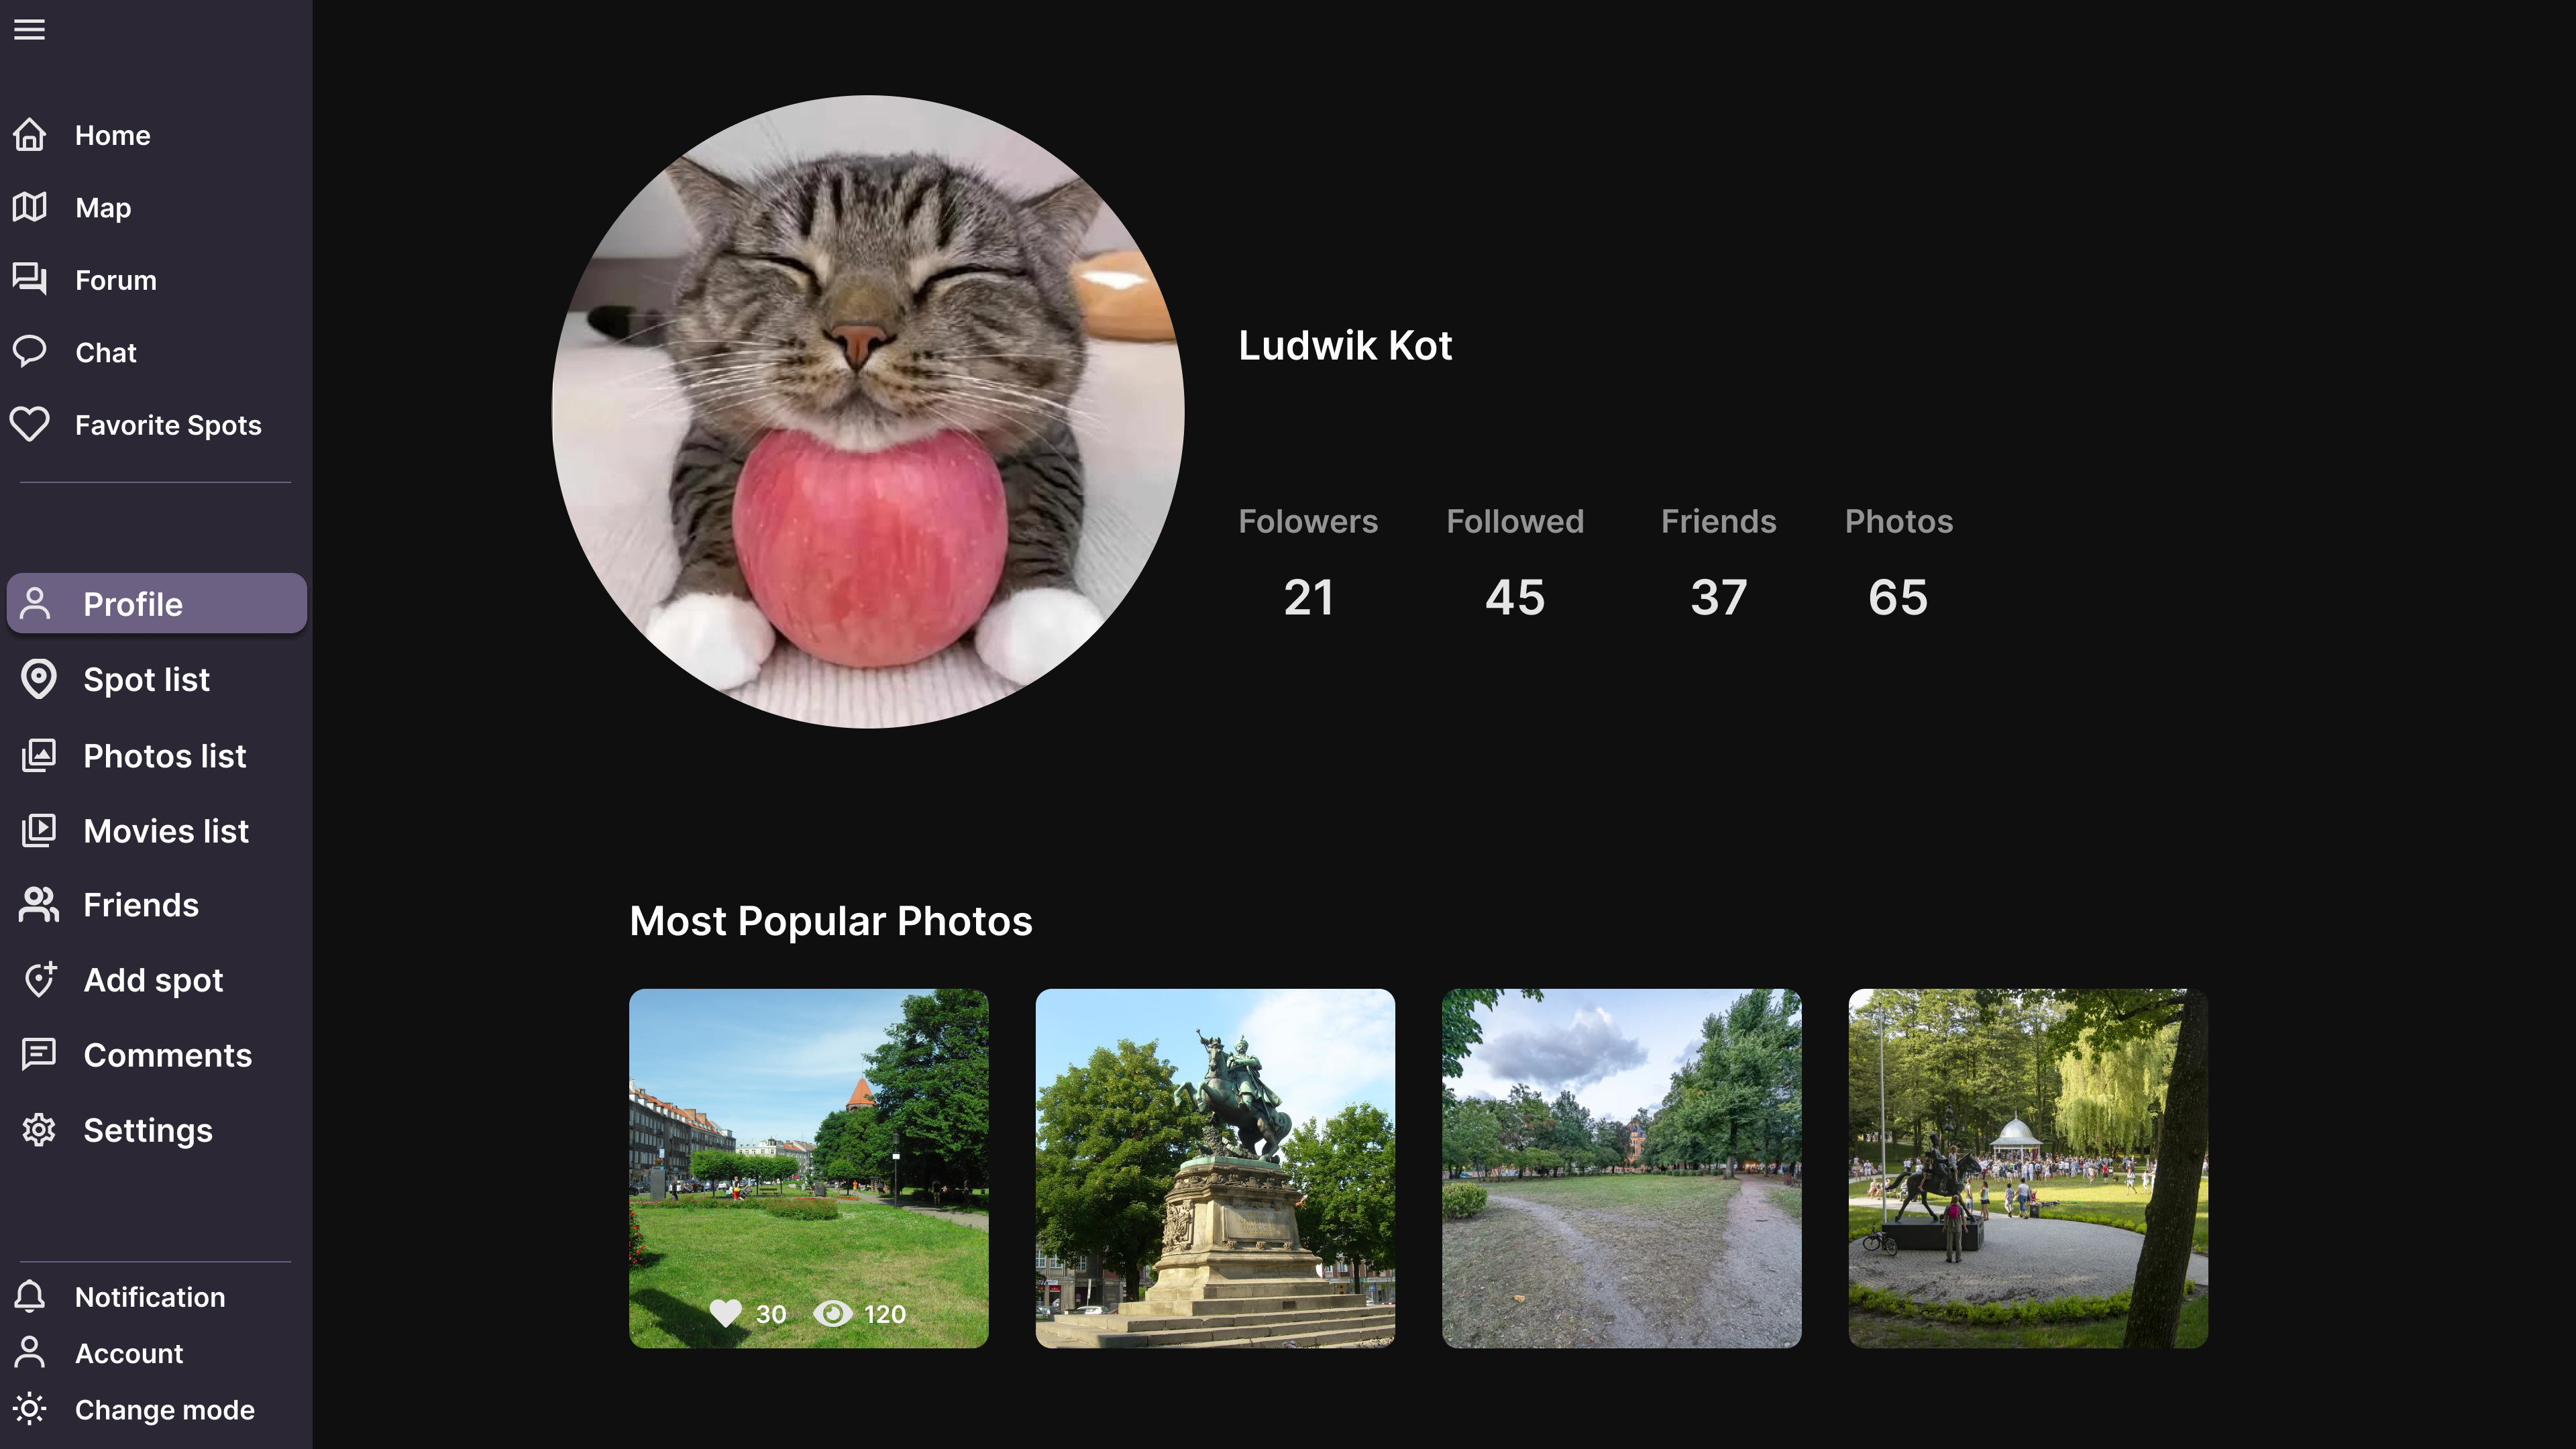
\includegraphics[width=1\textwidth]{attachments/projekt/architektura-interfejsu-uzytkownika/private-profile}
    \caption{Widok prywatny profilu}
    \label{img:private-profile}
\end{figure}
\begin{figure}[H]
    \centering
    \includegraphics[width=1\textwidth]{attachments/projekt/architektura-interfejsu-uzytkownika/public-profile}
    \caption{Widok publiczny profilu}
    \label{img:public-profile}
\end{figure}

\begin{figure}[H]
    \centering
    \includegraphics[width=1\textwidth]{attachments/projekt/architektura-interfejsu-uzytkownika/public-profile-followers}
    \caption{Lista obserwujących}
    \label{img:public-profile-followers}
\end{figure}
\begin{figure}[H]
    \centering
    \includegraphics[width=1\textwidth]{attachments/projekt/architektura-interfejsu-uzytkownika/public-profile-followed}
    \caption{Lista obserwowanych}
    \label{img:public-profile-followed}
\end{figure}

\begin{figure}[H]
    \centering
    \includegraphics[width=1\textwidth]{attachments/projekt/architektura-interfejsu-uzytkownika/public-profile-friends}
    \caption{Lista znajomych}
    \label{img:public-profile-friends}
\end{figure}
\begin{figure}[H]
    \centering
    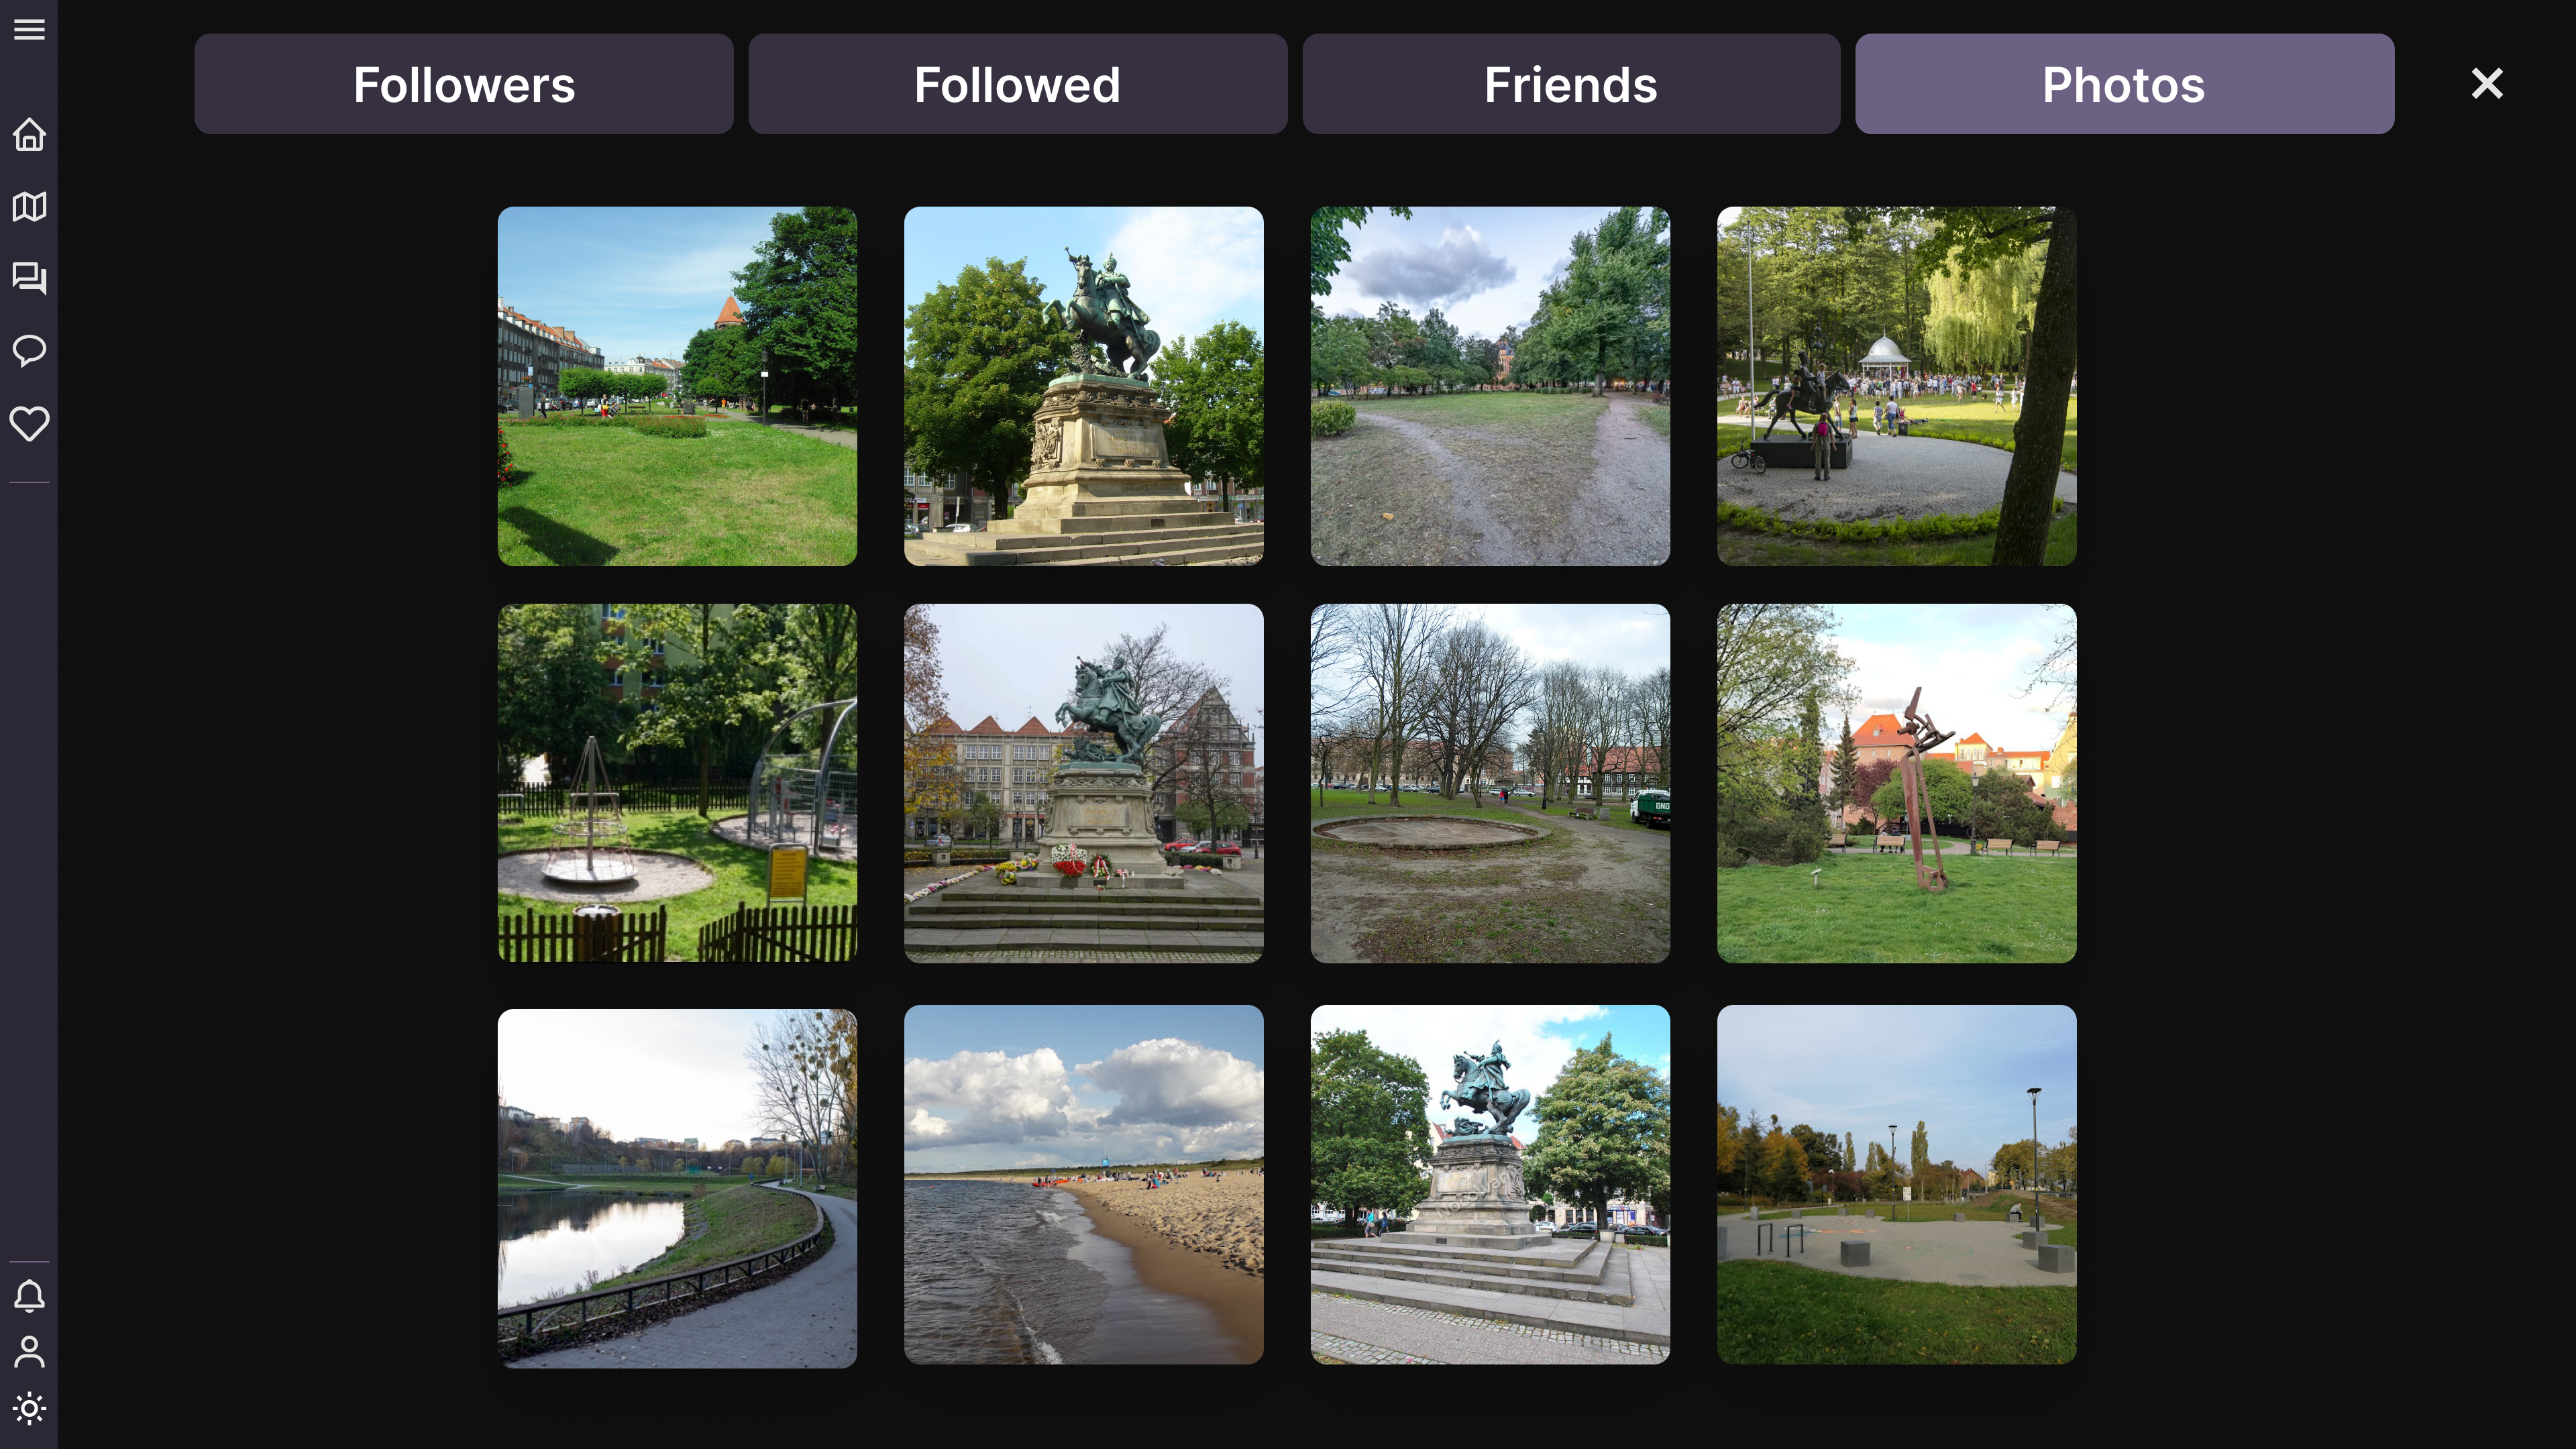
\includegraphics[width=1\textwidth]{attachments/projekt/architektura-interfejsu-uzytkownika/public-profile-photos}
    \caption{Lista zdjęć użytkownika}
    \label{img:public-profile-photos}
\end{figure}

\begin{figure}[H]
    \centering
    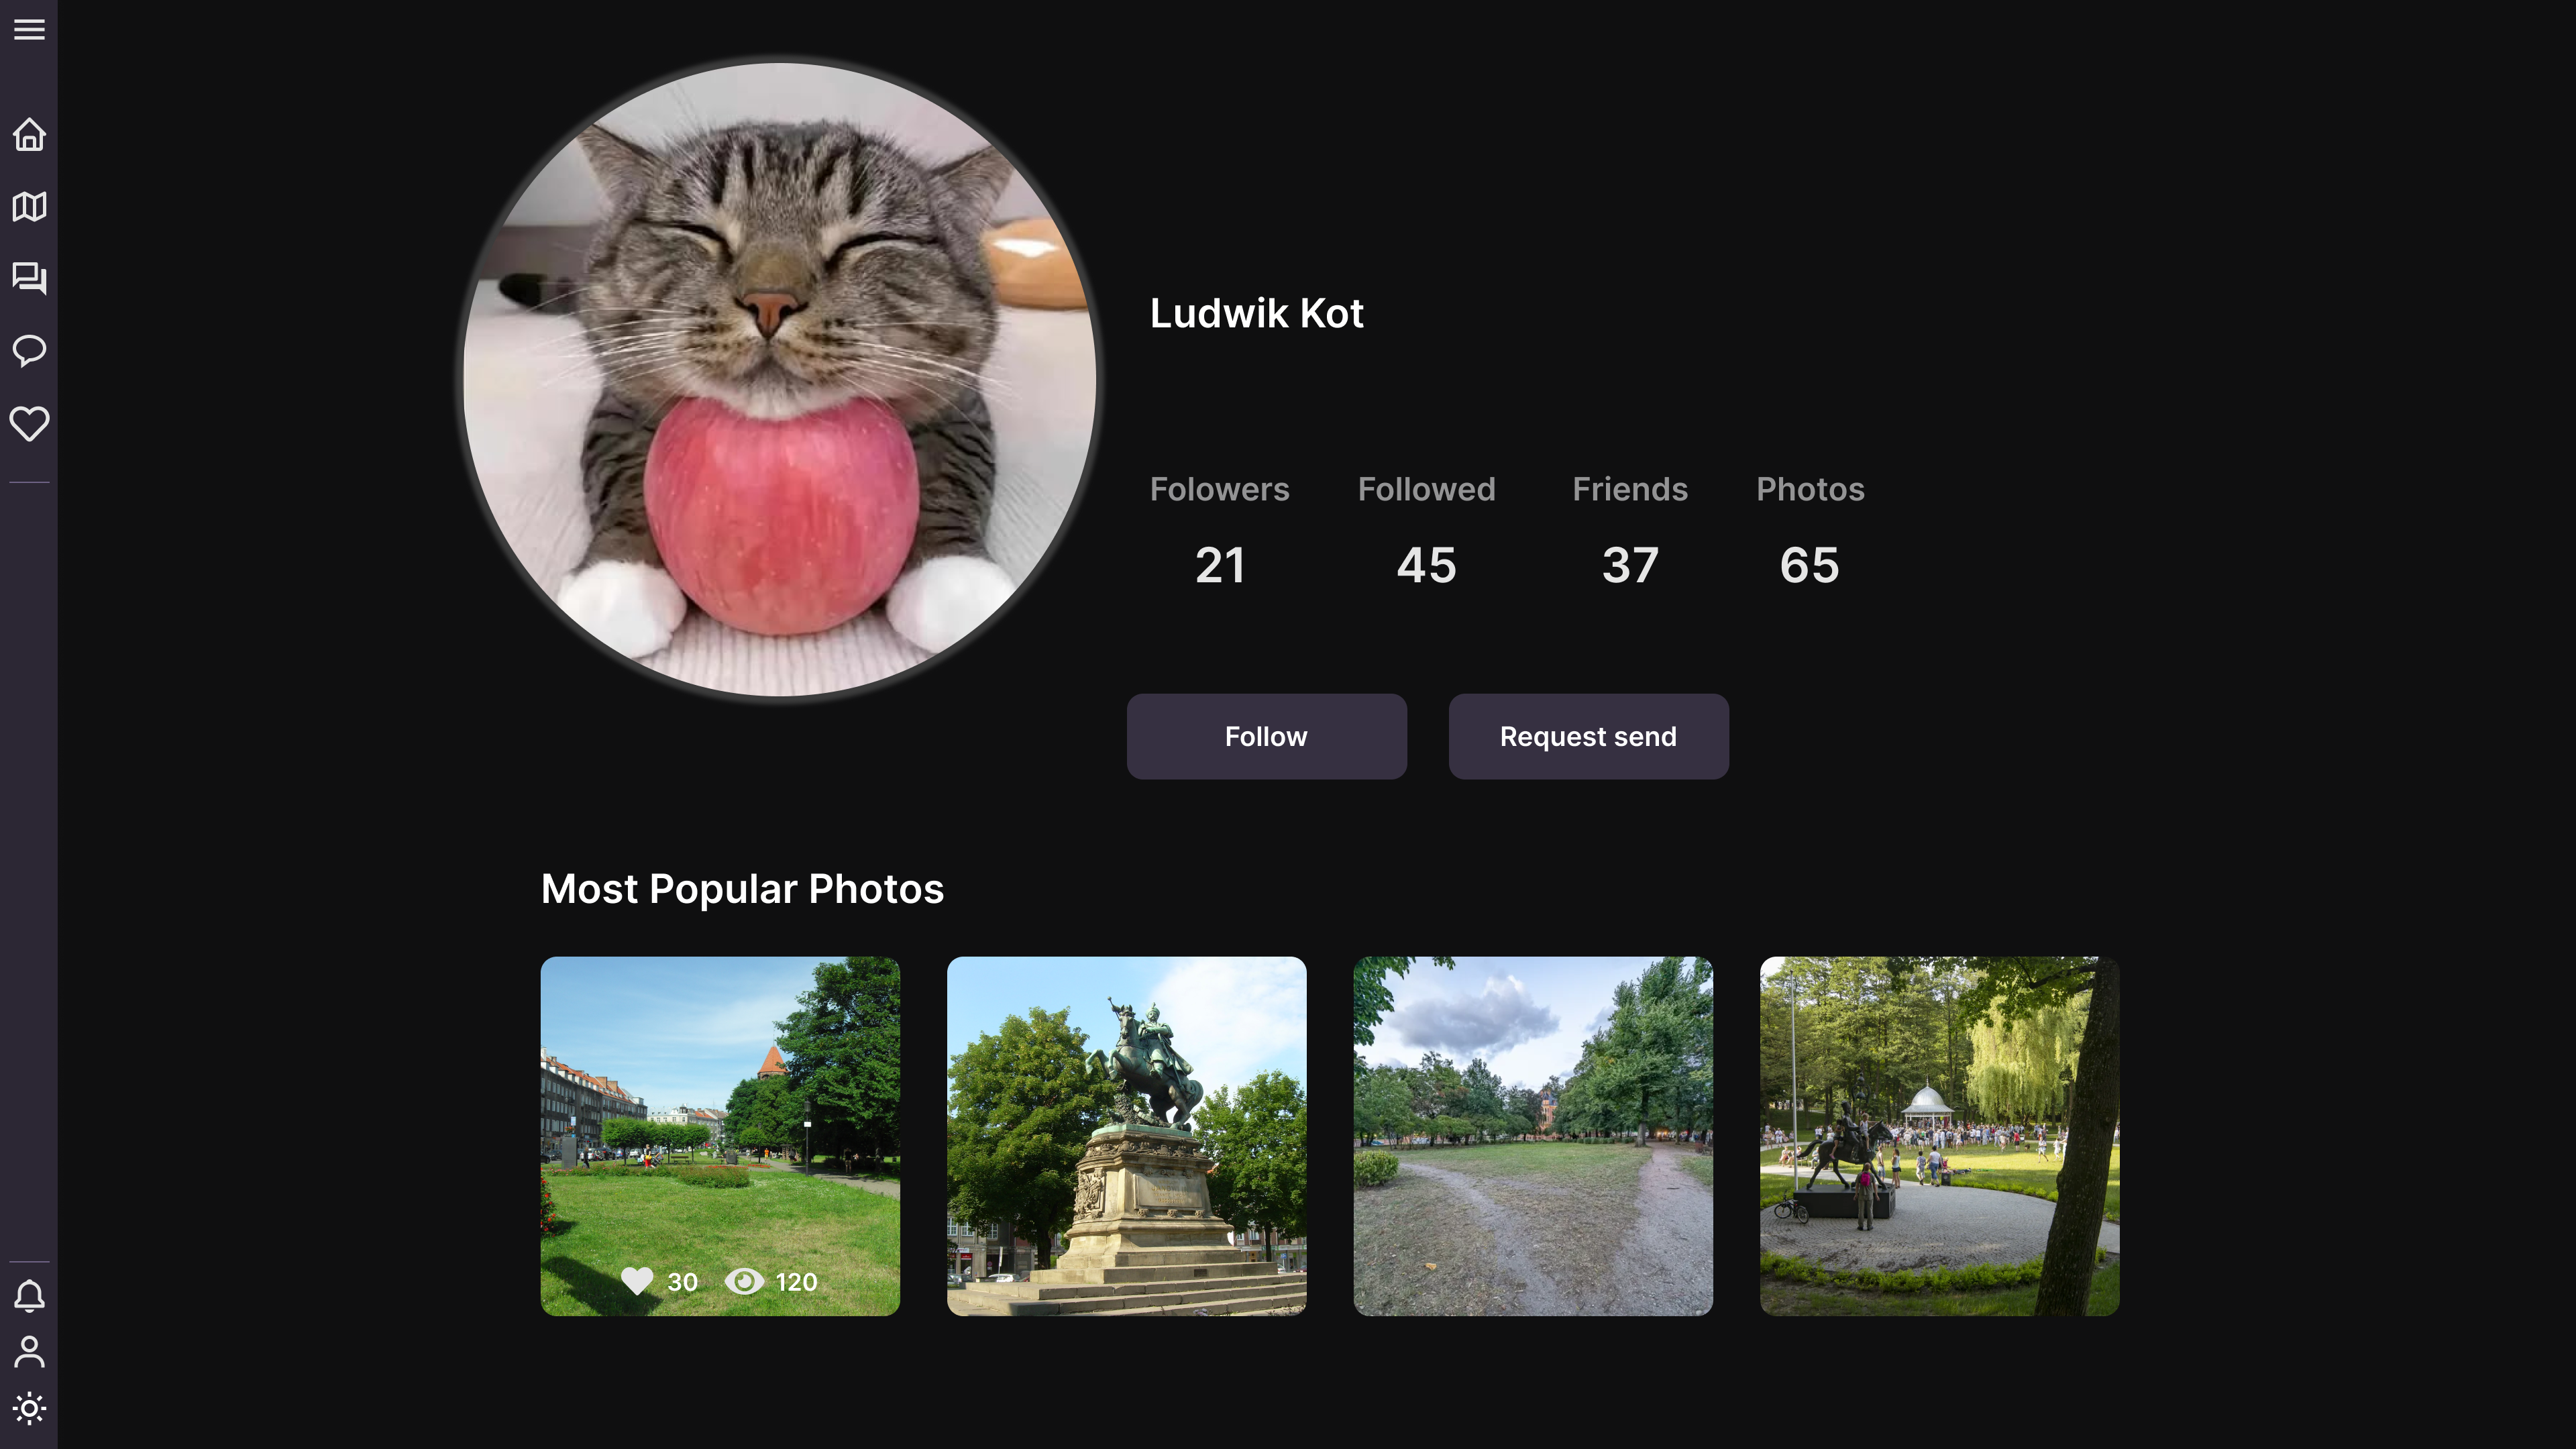
\includegraphics[width=1\textwidth]{attachments/projekt/architektura-interfejsu-uzytkownika/public-profile-request-send}
    \caption{Zaproszenie wysłane}
    \label{img:public-profile-request-send}
\end{figure}
\begin{figure}[H]
    \centering
    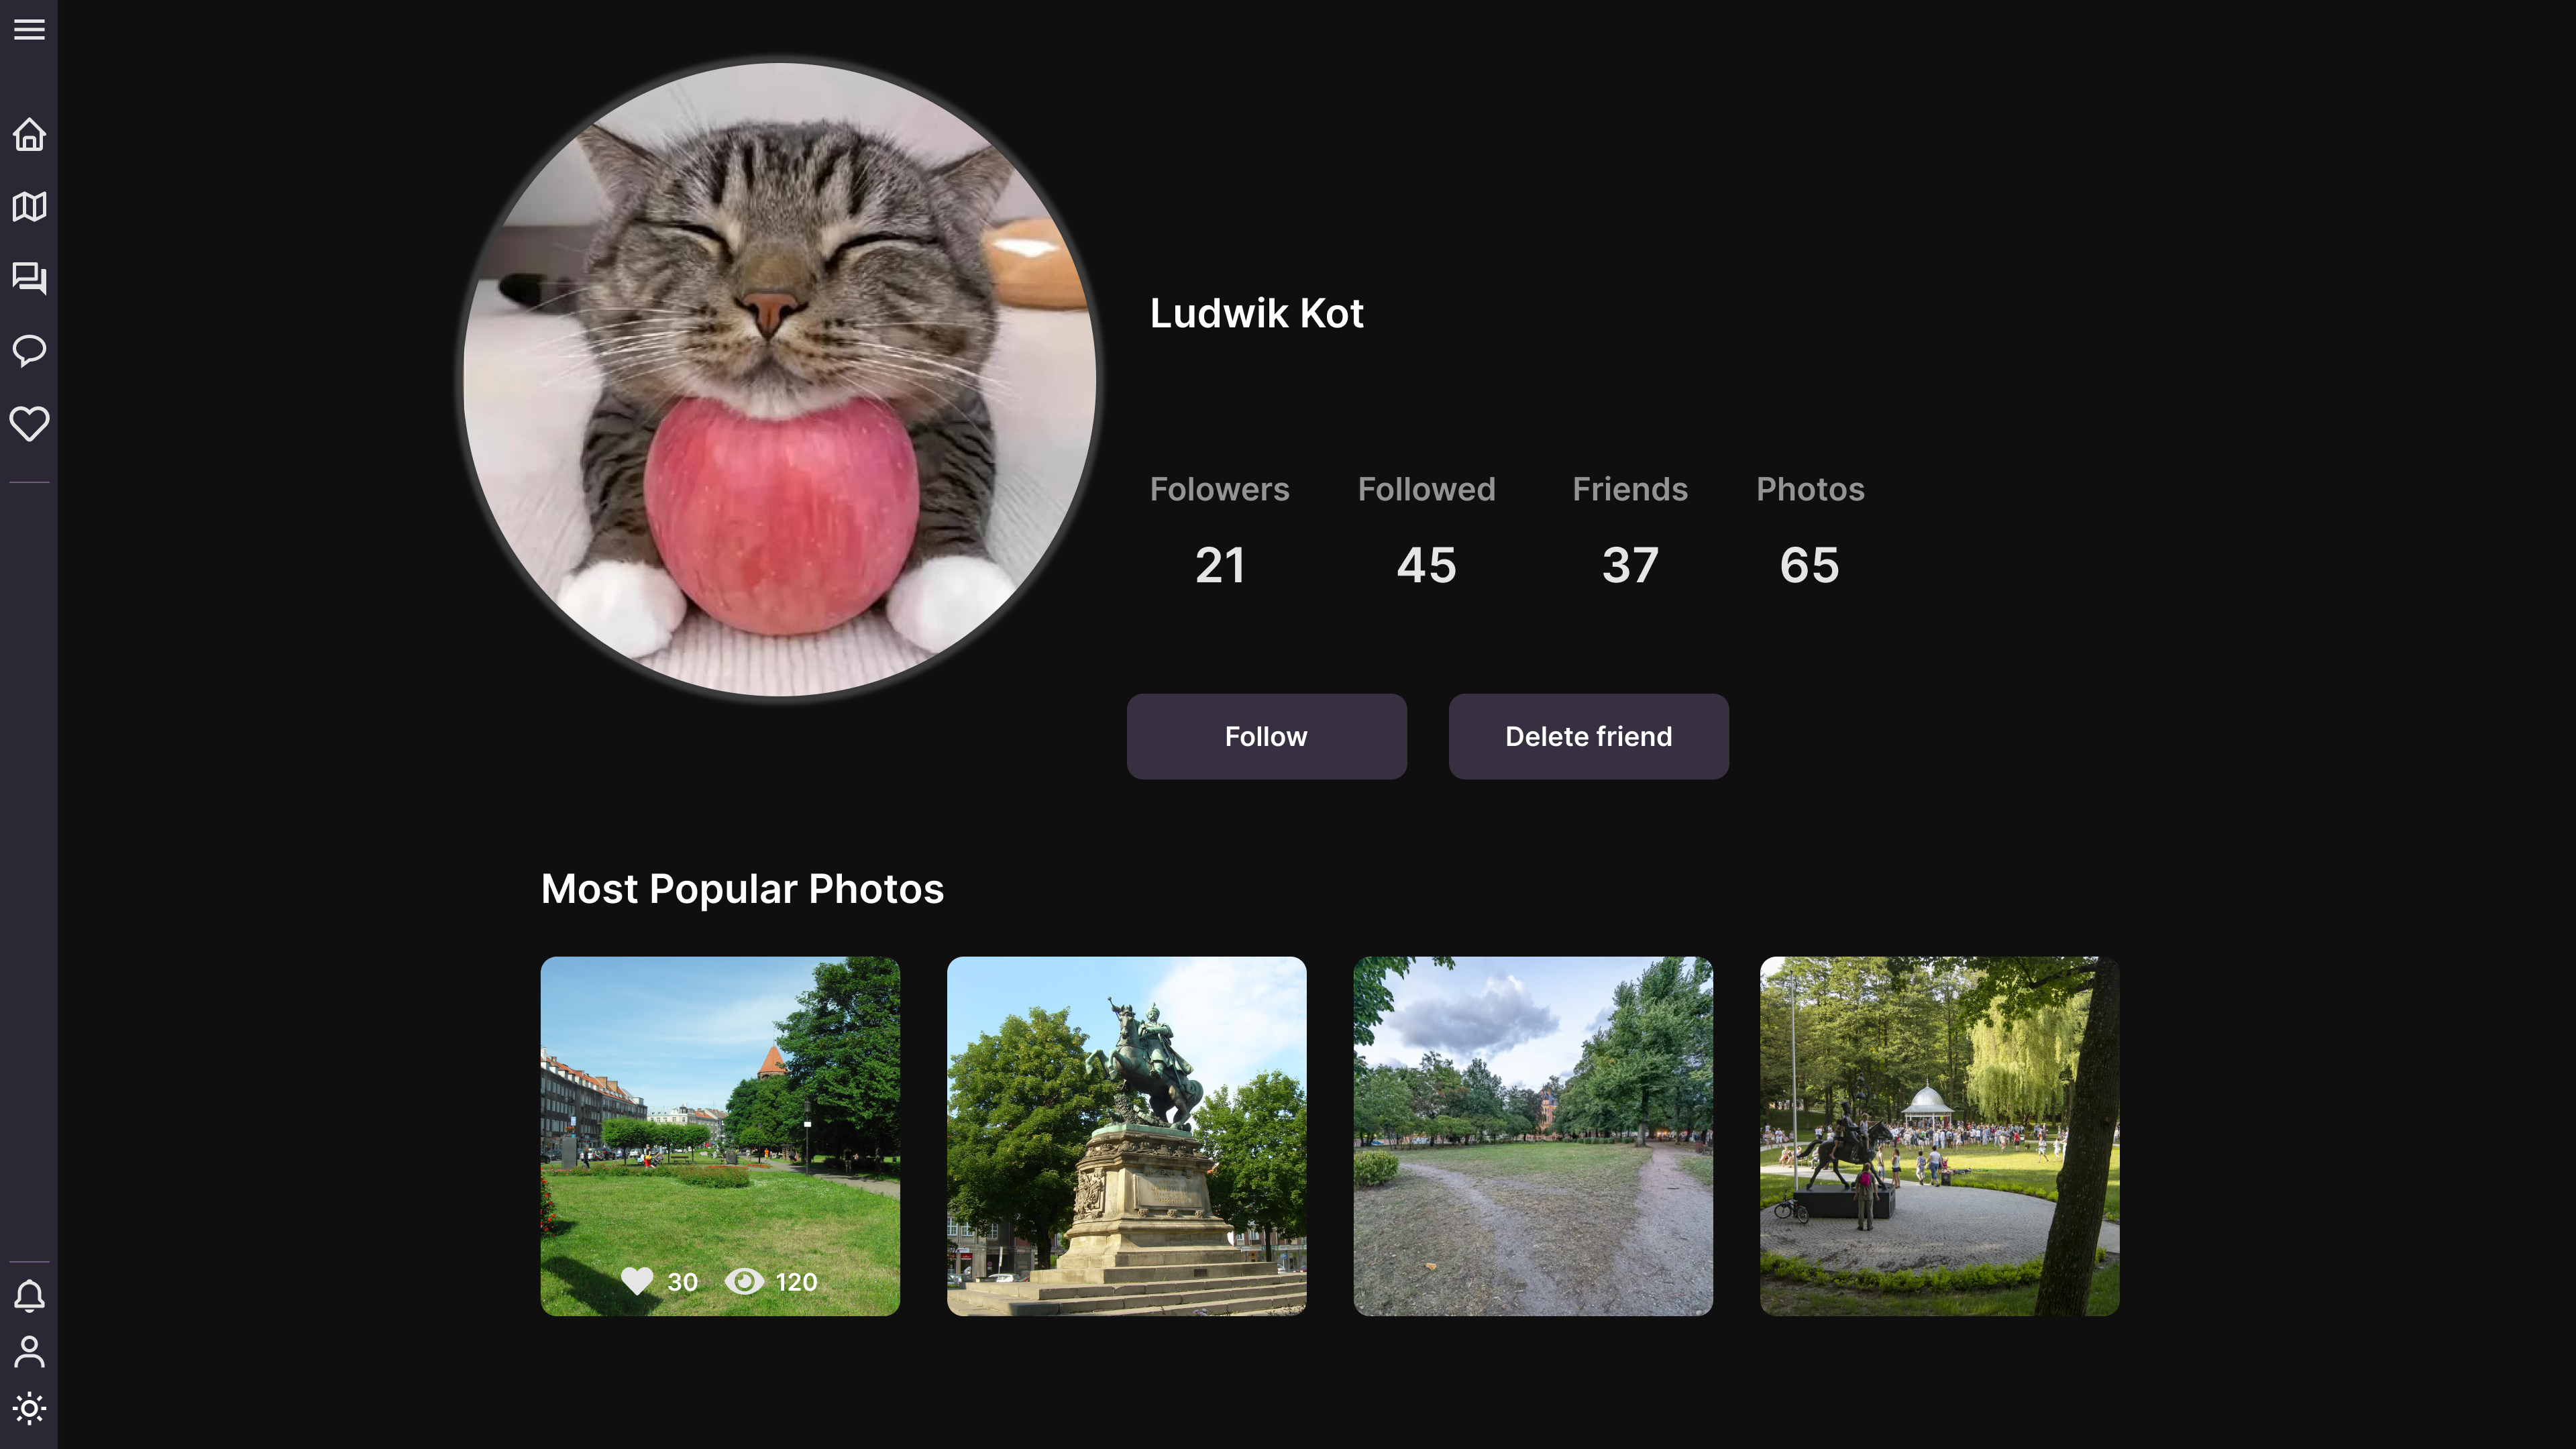
\includegraphics[width=1\textwidth]{attachments/projekt/architektura-interfejsu-uzytkownika/public-profile-remove-friend}
    \caption{Możliwość usunięcia z listy znajomych}
    \label{img:public-profile-remove-friend}
\end{figure}
\begin{figure}[H]
    \centering
    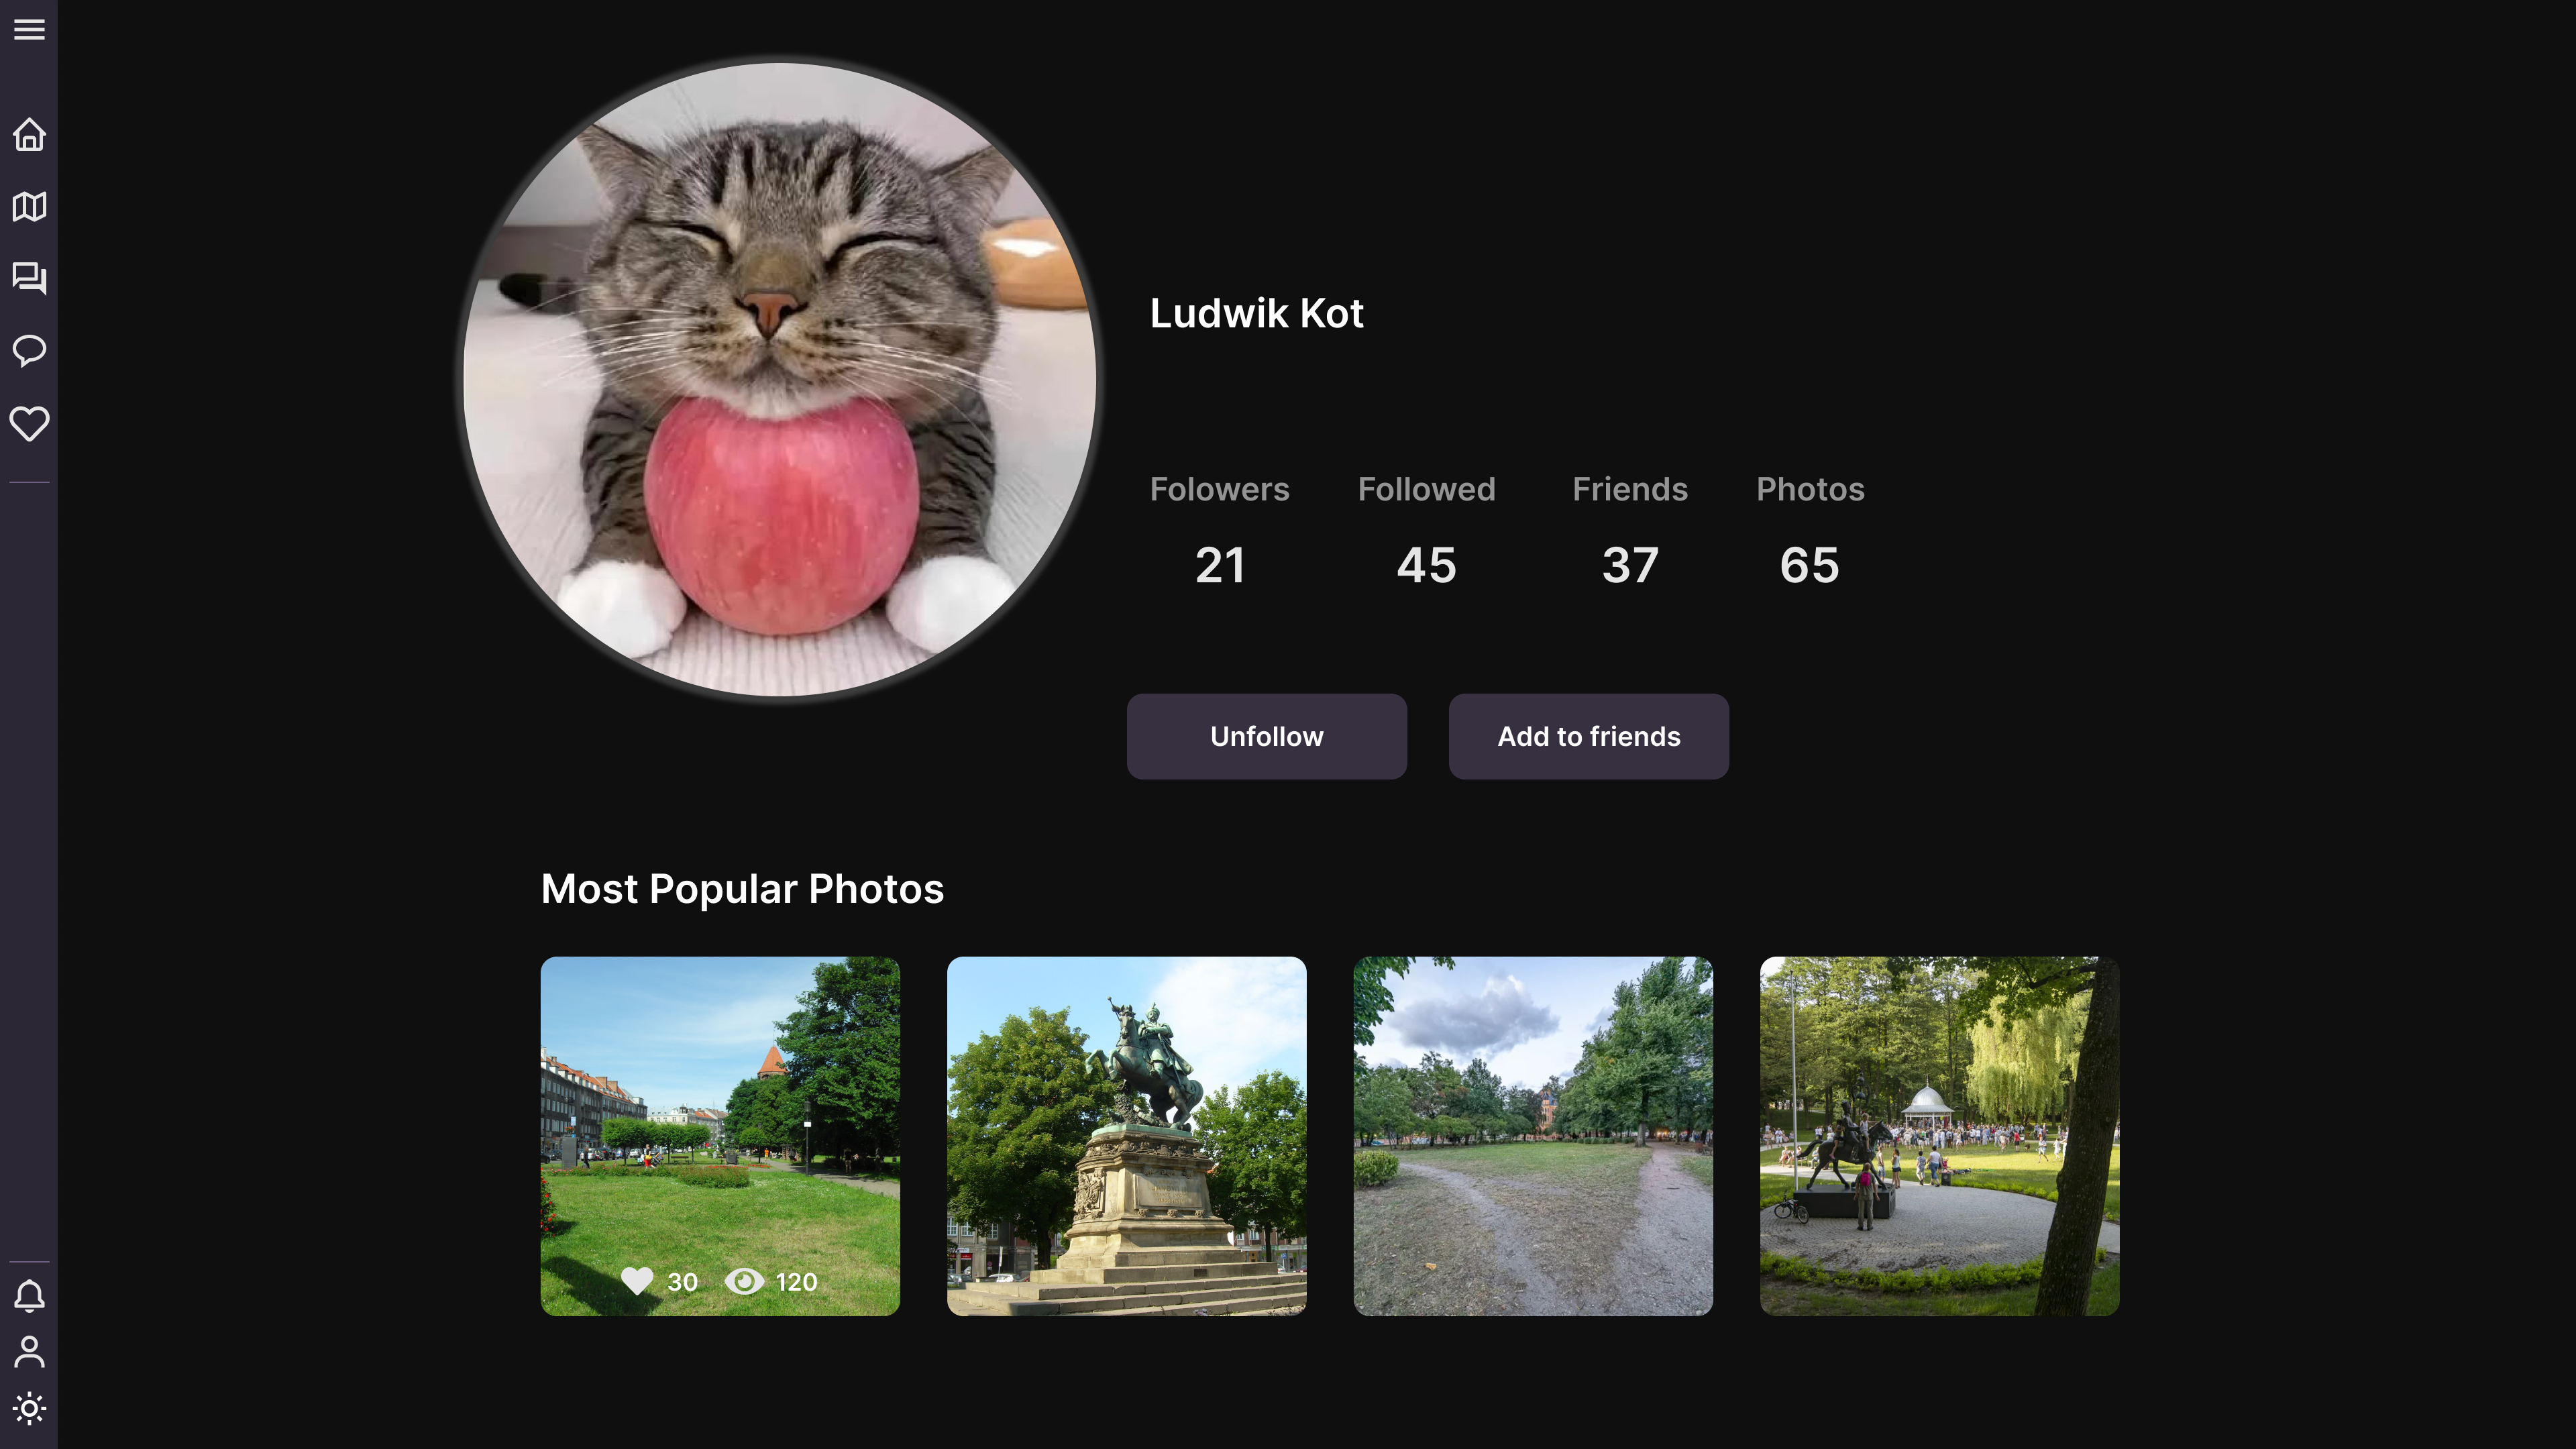
\includegraphics[width=1\textwidth]{attachments/projekt/architektura-interfejsu-uzytkownika/public-profile-unfollow}
    \caption{Możliwość zakończenia obserwowania}
    \label{img:public-profile-unfollow}
\end{figure}

\subsubsection{Spots list}

\begin{figure}[H]
    \centering
    \includegraphics[width=1\textwidth]{attachments/projekt/architektura-interfejsu-uzytkownika/spot-lists}
    \caption{Projekt strony z listą ulubionych spotów}
    \label{img:spot-lists}
\end{figure}

\subsubsection{Photos list}

\begin{figure}[H]
    \centering
    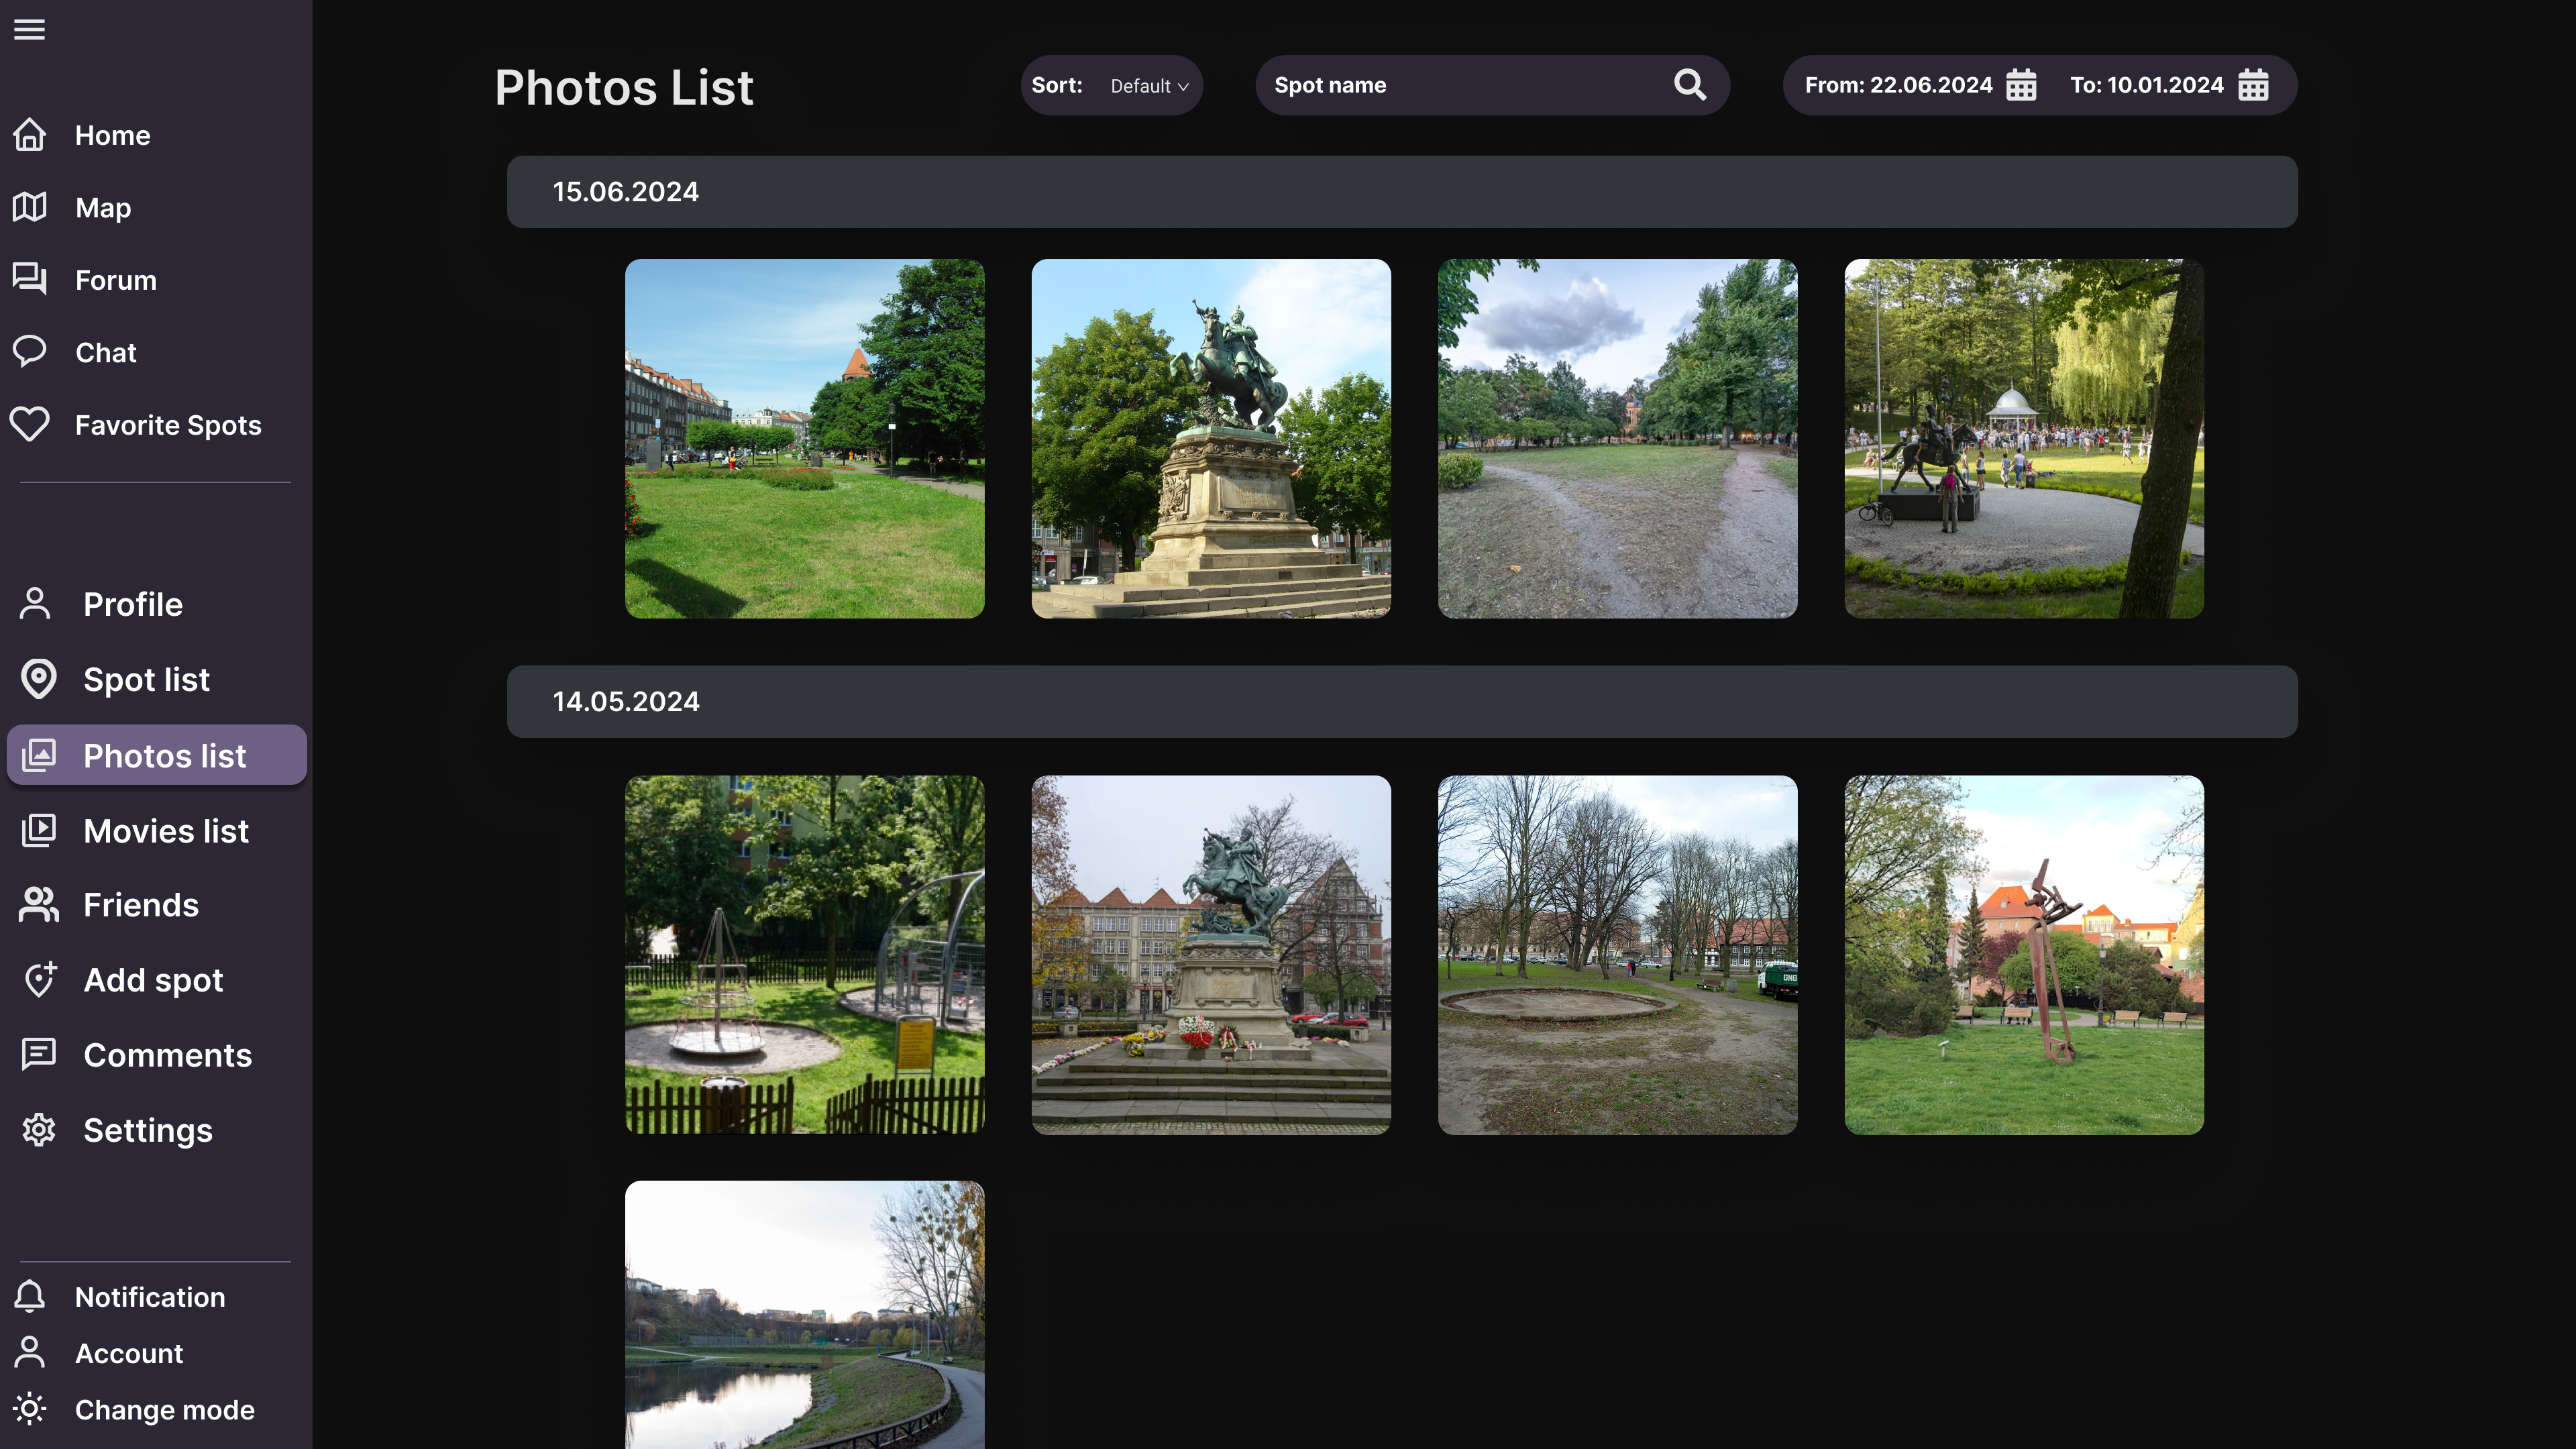
\includegraphics[width=1\textwidth]{attachments/projekt/architektura-interfejsu-uzytkownika/photos}
    \caption{Projekt strony z listą dodanych zdjęć}
    \label{img:photos}
\end{figure}

\subsubsection{Movies list}

\begin{figure}[H]
    \centering
    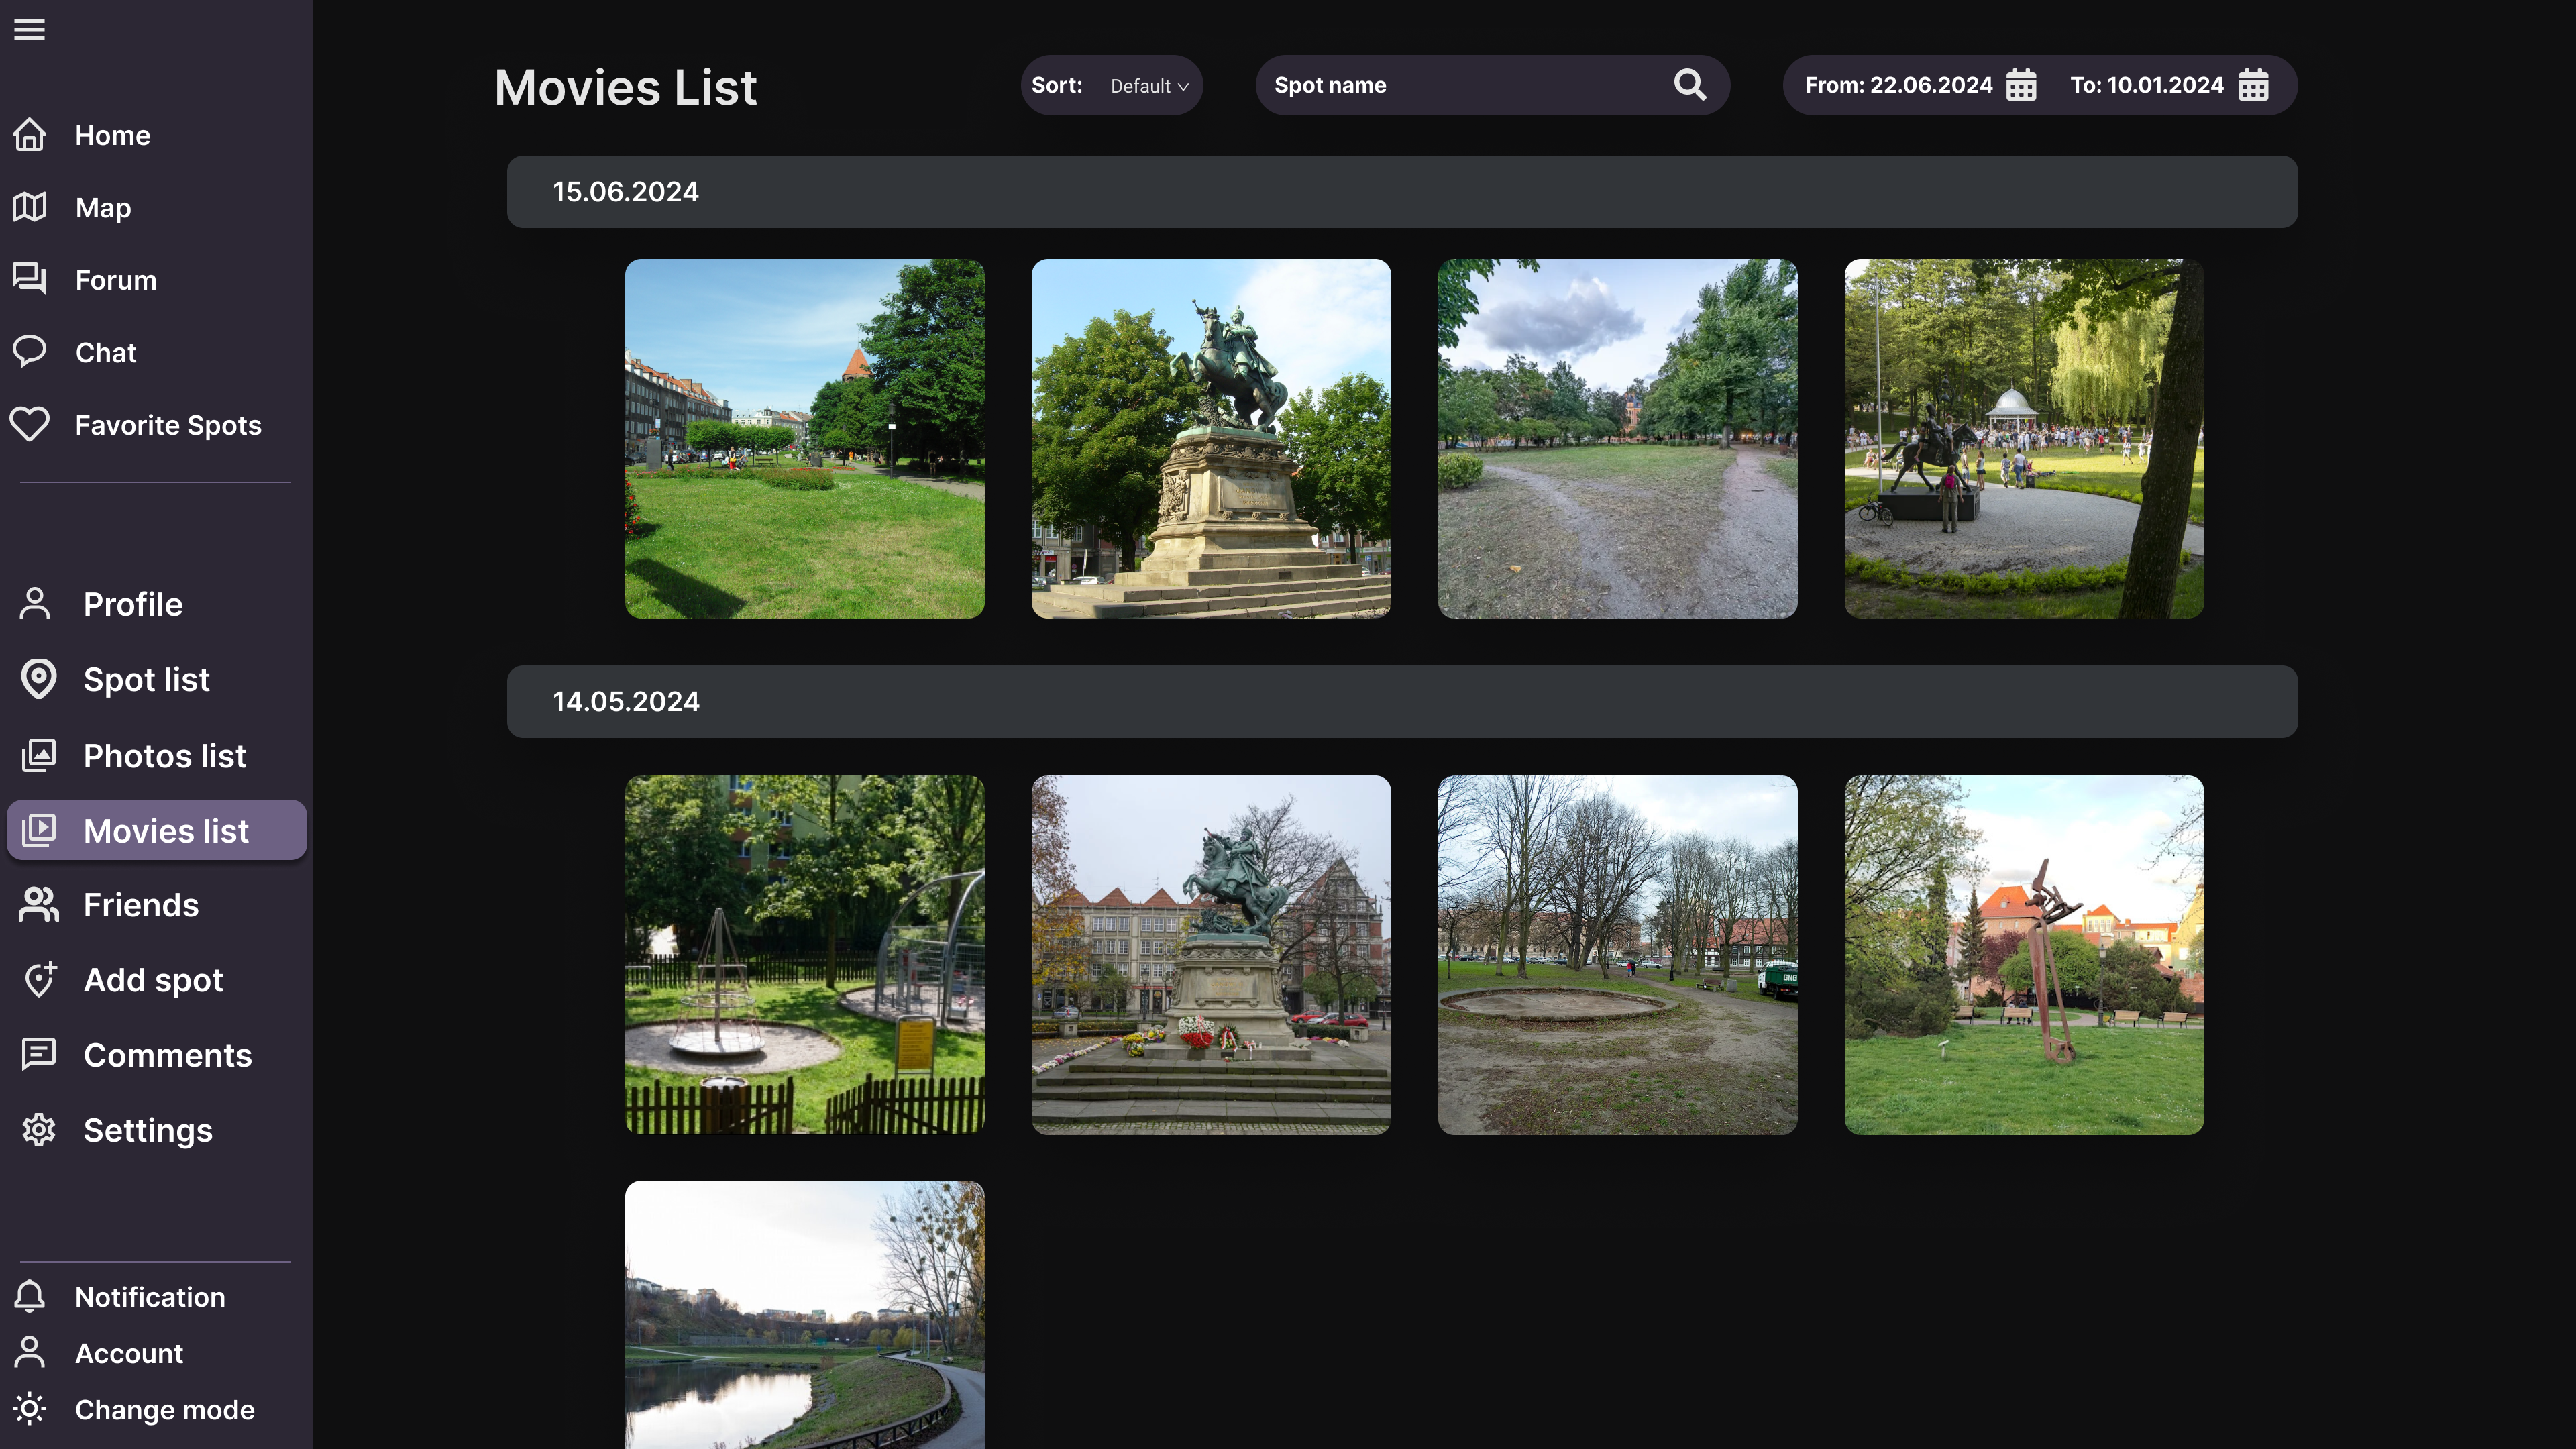
\includegraphics[width=1\textwidth]{attachments/projekt/architektura-interfejsu-uzytkownika/movies}
    \caption{Projekt strony z listą dodanych filmów}
    \label{img:movies}
\end{figure}

\subsubsection{Friends}

\begin{figure}[H]
    \centering
    \includegraphics[width=1\textwidth]{attachments/projekt/architektura-interfejsu-uzytkownika/friends}
    \caption{Projekt strony z listą znajomych}
    \label{img:friends}
\end{figure}

\subsubsection{Add spot}

\begin{figure}[H]
    \centering
    \includegraphics[width=1\textwidth]{attachments/projekt/architektura-interfejsu-uzytkownika/add-spot-list}
    \caption{Projekt strony z listą dodanych spotów}
    \label{img:add-spot-list}
\end{figure}

\begin{figure}[H]
    \centering
    \includegraphics[width=1\textwidth]{attachments/projekt/architektura-interfejsu-uzytkownika/add-spot-modal}
    \caption{Projekt strony z formularzem do dodania nowego spota}
    \label{img:add-spot-modal}
\end{figure}

\subsubsection{Comments}

\begin{figure}[H]
    \centering
    \includegraphics[width=1\textwidth]{attachments/projekt/architektura-interfejsu-uzytkownika/comments}
    \caption{Projekt strony z listą dodanych komentarzy}
    \label{img:comments}
\end{figure}

\subsubsection{Settings}

\begin{figure}[H]
    \centering
    \includegraphics[width=1\textwidth]{attachments/projekt/architektura-interfejsu-uzytkownika/settings}
    \caption{Projekt strony ustawień (1)}
    \label{img:settings}
\end{figure}

\begin{figure}[H]
    \centering
    \includegraphics[width=1\textwidth]{attachments/projekt/architektura-interfejsu-uzytkownika/settings-change-password}
    \caption{Projekt strony ustawień (2)}
    \label{img:settings-change-password}
\end{figure}